\documentclass[12pt]{article}
\usepackage{graphicx}
\usepackage{ragged2e}
\usepackage{array}
\usepackage{amsmath,xparse}
\usepackage{longtable}
\pagestyle{empty}
\newcolumntype{L}[1]{>{\raggedright\let\newline\\\arraybackslash\hspace{0pt}}m{#1}}
\newcolumntype{C}[1]{>{\centering\let\newline\\\arraybackslash\hspace{0pt}}m{#1}}
\newcolumntype{R}[1]{>{\raggedleft\let\newline\\\arraybackslash\hspace{0pt}}m{#1}}
\begin{document}
	\centering{\bf{KOLHAPUR INSTITUTE OF TECHNOLOGY'S}}\par
	{\bf{COLLEGE OF ENGINEERING (AUTONOMOUS),KOLHAPUR}}
	\par\noindent\rule{\textwidth}{0.4pt}
	
	\centering{\bf{FIRST YEAR B.Tech}}\par
	\centering{\bf{MID SEMESTER EXAMINATION}}\par
	\centering{\bf{EM1 (BSHM1)}}\par
	\begin{flushleft}
		Day and Date :{}\hspace{5.5cm}PRN:
	\end{flushleft}
	
	\begin{flushleft}
		Time :{}\hspace{7cm}Max Marks:{30}\\
	\end{flushleft}
	\noindent\rule{\textwidth}{0.1pt}
\begin{flushleft}
	{\bf Instructions:}\\
	{\hspace{0.5cm} \bf IMP: Verify that you have received question paper with correct course, code, branch, etc}\\
	\hspace{1cm}i) All Questions are Compulsory\\
	\hspace{1cm}ii)Figure to right indicate full marks\\
	\hspace{1cm}iii)Assume suitable data wherever necessary\\
\end{flushleft}

	\begin{flushleft}
	\bf{QNo}\hspace{1.2cm} \bf{Question} \hspace{5.5cm}  \bf{Marks} \hspace{0.2cm} \bf{CO} \hspace{0.2cm}	\bf{BL}	
	
\end{flushleft} 
	\begin{longtable}{|L{1cm}|L{8cm}|C{1cm}|C{1cm}|C{1cm}|}\hline
		\bf{1}. & \bf{Attempt} \bf1 \bf{out} of \bf2 & \bf10  & & \\ \hline
				1.A & What is the default Value ? \newline
					
		A)val1\newline
		B)val2\newline
		C)val3\newline
		D)val4 &
		9 &
		CO2&
		1 \\ \hline
		
				1.B & The Value of Suppose 2+3= \newline
					
		A)3\newline
		B)4\newline
		C)6\newline
		D)7 &
		9 &
		CO2&
		1 \\ \hline
		
		
	\end{longtable}

	\begin{longtable}{|L{1cm}|L{8cm}|C{1cm}|C{1cm}|C{1cm}|}\hline
	\bf2. & \bf{Attempt} \bf{1} \bf{out of} \bf{2} & \bf{10}  & & \\ \hline





		2.A &
	What is mathematic \newline
			
	 &  9 & CO4 & 2\\ \hline
		2.B &
	what is the value of this shit. \newline
			
	 &  9 & CO5 & 4\\ \hline
	\end{longtable}


\begin{longtable}{|L{1cm}|L{8cm}|C{1cm}|C{1cm}|C{1cm}|}\hline
	\bf3. & \bf{Attempt} \bf{1} \bf{out of} \bf{2} & \bf{10}  & & \\ \hline





		3.A &
	what is in this question again whith ease \newline
			
	 &  9 & CO4 & 2\\ \hline
		3.B &
	Image type question \newline
			\begin{center}
		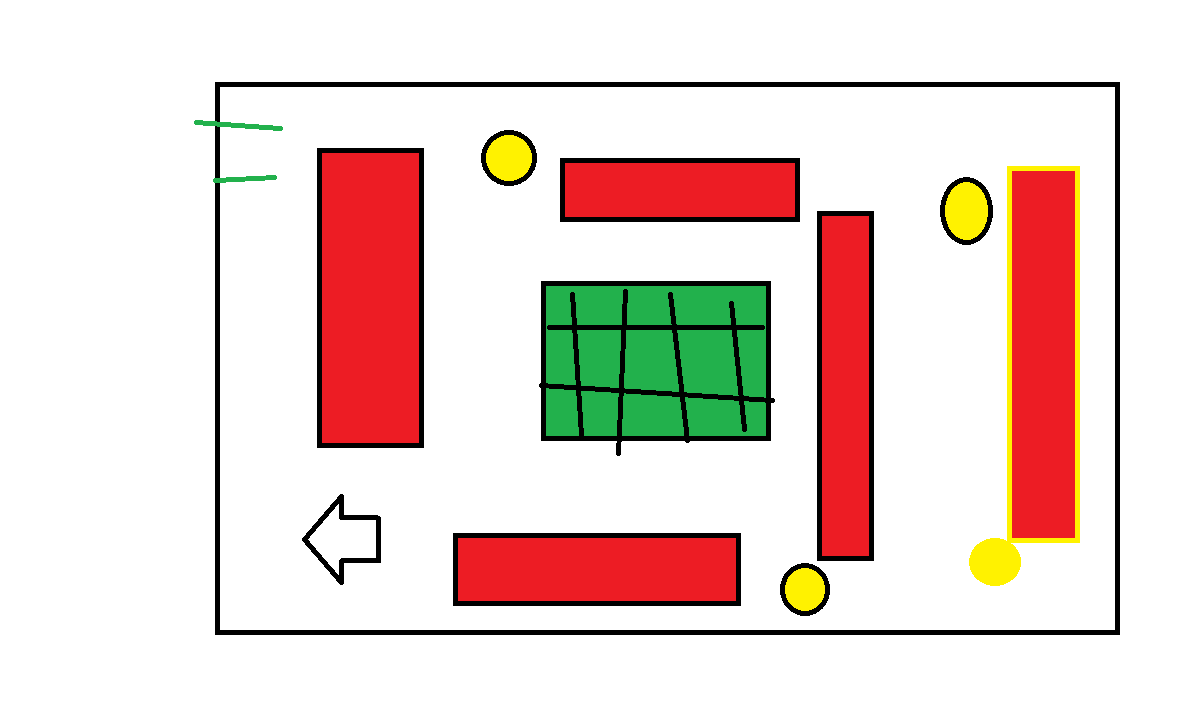
\includegraphics[width=4cm,height=3cm]{media/diagrams/2020/05/27/gameidea.png}\\\bf{Figure }\bf3.B		
	\end{center}
		
	 &  9 & CO3 & 2\\ \hline
	\end{longtable}



\end{document}
	
	